\documentclass[11pt]{article}

% ─────────────────────────── packages ───────────────────────────
\usepackage[T1]{fontenc}
\usepackage[utf8]{inputenc}
\usepackage[a4paper,margin=2.2cm]{geometry}
\usepackage{charter}
\usepackage[scaled=0.92]{helvet}
\usepackage{xcolor}
\usepackage{eurosym}
\usepackage{titlesec}
\usepackage{booktabs}
\usepackage{enumitem}
\usepackage{array}
\usepackage{graphicx}
\usepackage{fancyhdr}
\usepackage[most]{tcolorbox}
\usepackage{parskip}
\usepackage[hidelinks]{hyperref}

% ─────────────────────────── palette ────────────────────────────
\definecolor{accent}{HTML}{2563EB}
\definecolor{darkbg}{HTML}{0A0F1A}
\definecolor{ink}{HTML}{111827}
\definecolor{ink2}{HTML}{4B5563}
\definecolor{ink3}{HTML}{6B7280}
\definecolor{rule}{HTML}{E5E7EB}
\definecolor{green}{HTML}{059669}
\definecolor{amber}{HTML}{B45309}
\definecolor{redx}{HTML}{DC2626}
\definecolor{accentbg}{HTML}{EFF6FF}
\definecolor{greenbg}{HTML}{ECFDF5}

\hypersetup{colorlinks=true, linkcolor=accent, urlcolor=accent, citecolor=accent}
\renewcommand{\familydefault}{\rmdefault}

% ─────────────────────────── headings ───────────────────────────
\titleformat{\section}{\sffamily\large\bfseries\color{ink}}{\thesection}{0.6em}{}
\titleformat{\subsection}{\sffamily\normalsize\bfseries\color{accent}}{\thesubsection}{0.6em}{}
\titlespacing*{\section}{0pt}{16pt}{6pt}
\titlespacing*{\subsection}{0pt}{11pt}{3pt}

% ─────────────────────────── header/footer ──────────────────────
\pagestyle{fancy}
\fancyhf{}
\renewcommand{\headrulewidth}{0.4pt}
\renewcommand{\headrule}{\color{rule}\hrule height 0.4pt}
\fancyhead[L]{\footnotesize\sffamily\color{ink3}AIDER \textbar\ AI-Driven Energy Research}
\fancyhead[R]{\footnotesize\sffamily\color{ink3}Meetup Record \& Briefing \textbar\ 13 June 2026}
\fancyfoot[C]{\footnotesize\sffamily\color{ink3}\thepage}

% ─────────────────────────── helpers ────────────────────────────
\newcommand{\stat}[1]{{\sffamily\bfseries\color{accent}#1}}
\newcommand{\src}[1]{{\footnotesize\color{ink3}[#1]}}

% callout box
\newtcolorbox{takeaway}{
  colback=accentbg, colframe=accent, boxrule=0.8pt, arc=2pt,
  left=8pt, right=8pt, top=6pt, bottom=6pt, fontupper=\small}
\newtcolorbox{solvebox}{
  colback=greenbg, colframe=green, boxrule=0.8pt, arc=2pt,
  left=8pt, right=8pt, top=6pt, bottom=6pt, fontupper=\small}

\setlist[itemize]{leftmargin=1.2em, itemsep=2pt, topsep=2pt}
\setlist[enumerate]{leftmargin=1.4em, itemsep=2pt, topsep=2pt}

% ═════════════════════════════════════════════════════════════════
\begin{document}

% ─────────────────────────── title block ────────────────────────
\begin{tcolorbox}[colback=darkbg, colframe=darkbg, arc=3pt, left=18pt, right=18pt, top=14pt, bottom=14pt]
  {\sffamily\footnotesize\color{accent}\bfseries DIAMOND OPEN ACCESS \textbullet\ EDITORIAL BRIEFING}\\[4pt]
  {\sffamily\LARGE\bfseries\color{white} AI-Driven Energy Research (AIDER)}\\[5pt]
  {\sffamily\small\color{white!75} The problems we solve, how we win, and where we are.}\\[8pt]
  {\sffamily\footnotesize\color{white!60} First editors' online meetup \textbullet\ Saturday 13 June 2026 \textbullet\ 8:00--8:30 pm Beijing (UTC+8)}
\end{tcolorbox}

\vspace{4pt}

% ─────────────────────── meeting discussion summary (prepended) ───────────────────────
\section*{Meeting Discussion Summary}
\vspace{-3pt}
{\footnotesize\sffamily\color{ink3}First editors' online meetup \textbullet\ Saturday 13 June 2026, 8:00--8:35 pm Beijing (UTC+8) \textbullet\ via Zoom}

\vspace{4pt}
{\small
\textbf{Present (active editors).} Jianou Jiang (Oxford, chair) \textbullet\ Raul Adriaensen (Imperial College London) \textbullet\ Jingda Wu (Kyoto University) \textbullet\ Dr.\ Feng Wei (CAICT / MIIT). Jianou noted that four editors are actively contributing, while several others lend their names to build the journal's early credibility.

\textbf{Walkthrough.} After introductions, Jianou presented this briefing --- the old problems (poor reproducibility, double payment, no home for individuals), the new ones (undocumented AI use; papers growing exponentially while referee capacity grows linearly), the competitor lessons (JOSS rejected by Web of Science for low-rigour ``user-guide'' papers; Distill closed in 2021 from volunteer burnout; MDPI / Hindawi delisted for accepting too much), and the short- and long-term plan.

\textbf{Key discussion points.}
\begin{itemize}[leftmargin=1.1em, itemsep=1.5pt, topsep=2pt]
\item \textbf{Reputation is fragile} (Raul). One weak early review or a retraction would sink trust quickly --- launch-stage review quality is existential. Lean on automated repository testing \emph{and} genuinely trustworthy papers.
\item \textbf{Two-tier ``middle-ground'' rollout} (Jianou). Start with a low bar to welcome submissions, but do \emph{not} auto-index them to Google Scholar / Web of Science; once indexed and with loyal contributors, invite revised resubmissions into the high-quality tier. Agreed as a sensible, acceptable-risk path.
\item \textbf{Who pays \& the moat} (Raul). Keep it free for individuals, but consider a modest fee for institutions (which are government-funded) to subsidise independent researchers. The real moat is the full transparency of each repository's AI research process --- valuable data for improving AI agents and for ``selling the acceleration of trustworthy research'' to governments and funders.
\item \textbf{Funding route} (Jianou). Pursue a postdoc and supervisor / professor collaborations so that government\,$\rightarrow$\,university\,$\rightarrow$\,platform funding flows when their students publish; also target the large body of unpublished postgraduate and small-scale work.
\item \textbf{Reviewers want community} (Raul). Offer top reviewers individual meetings and, eventually, a conference that convenes leading people; invite senior figures to future sessions. Avoid spammy mass emails --- reach people personally and build trust through regular meetings.
\item \textbf{Usability friction} (Jingda Wu). The reproducibility script and submission flow are currently harder than submitting to high-impact journals; simplify without lowering quality. Jianou: the GitHub agent is buggy (an easy fix); how much reproducibility to require is a spectrum to settle once 10--50 papers are in.
\item \textbf{Recruit senior back-catalogues} (Feng Wei). Engage established professors who lack the new tools, onboard their students, run workshops, and republish or extend strong older papers with reproducibility and new material --- raising their visibility.
\end{itemize}

\textbf{Agreed next steps.}
\begin{itemize}[leftmargin=1.1em, itemsep=1.5pt, topsep=2pt]
\item Secure the ISSN ($\sim$2 months out) and remaining certificates before any wider outreach; until then, grow only through personal networks.
\item Fix the GitHub submission / reproducibility tooling to lower the barrier to submit.
\item Raul to complete the review of the fifth paper so it can be published.
\item Reconvene after ISSN news to decide the promotion strategy and next moves.
\end{itemize}
}
\clearpage

{\small\color{ink2} This briefing frames the gap AIDER exists to close, the strategy to climb from a free new journal to a recognised one, who our first authors and reviewers are, and our current status. \textbf{Every quantitative claim is sourced}; references are listed on the final page.}

% ═════════════════════════════════════════════════════════════════
\section{The Problems We Are Solving}

Scholarly publishing was already strained before generative AI. The GPT era did not create a new system --- it poured fuel on the cracks of the old one. We group the problems into the \textbf{pre-GPT structural failures} and the \textbf{post-GPT accelerants}.

\subsection{Old problems (pre-GPT era)}

\textbf{(a) Research is not open or reproducible enough --- so it is not reused.}
Findings stay locked in static PDFs while the code and data that produced them are never shared. In a landmark \emph{Nature} survey of 1{,}576 researchers, \stat{>70\%} had tried and failed to reproduce another scientist's experiments and \stat{>50\%} failed to reproduce their \emph{own}; \stat{52\%} called it a ``significant'' reproducibility crisis. \src{1} Even where sharing is mandated, it rarely happens: of 204 \emph{Science} papers under a compulsory data/code policy, only \stat{44\%} of authors supplied materials and results were independently reproducible for just \stat{26\%}. \src{2} Data evaporates with time --- its availability falls \stat{17\% per year} of article age, so barely \stat{$\sim$6\%} of 20-year-old datasets remain obtainable. \src{3} The net effect: most published research cannot be built upon, only cited.

\textbf{(b) Authors and readers pay --- for value the publisher did not add.}
The peer reviewers work for free, the authors write for free, yet the global STM publishing market is worth \stat{$\sim$\$19\,billion} a year. \src{6} Five publishers control \stat{>50\%} of all papers, \src{7} and they extract margins a tech monopoly would envy: Elsevier's parent RELX posted a \stat{38\%} operating margin in 2023. \src{8} To publish open access in a Nature journal costs \stat{\$11{,}390} (\euro9{,}500) per article --- a fee that has since risen above \$12{,}000. \src{5} Annual open-access fees paid to just six publishers \stat{tripled from \$0.91\,bn to \$2.54\,bn} between 2019 and 2023. \src{9} Readers without an institution hit paywalls; authors without a grant are priced out.

\textbf{(c) Independent researchers and developers have no high-quality home.}
A solo developer or an unfunded researcher with excellent, fully reproducible work faces a brutal choice: pay a four-figure APC, sign their copyright away to a paywall, or sink into a predatory venue. Free, no-fee ``diamond'' journals do exist --- an estimated \stat{17{,}000--29{,}000} of them, carrying \stat{8--9\%} of all articles --- but they are small (median \stat{$\sim$23 articles/year}), volunteer-run, and most are not even indexed. \src{10} There is no respected, reproducibility-first venue built for the individual contributor.

\subsection{New problems (the post-GPT accelerants)}

\textbf{(a) AI-assisted research is undocumented --- the process is a black box.}
AI is now woven through writing, coding, and analysis, yet almost none of it is recorded. Excess-vocabulary analysis of 15\,million biomedical abstracts shows at least \stat{13.5\%} of 2024 abstracts were LLM-processed --- up to \stat{40\%} in some subfields. \src{11} It has reached peer review too: \stat{6.5--16.9\%} of text in AI-conference reviews showed signs of LLM generation. \src{12} This matters because the tools are unreliable in ways only a process log would catch: ChatGPT (GPT-3.5) \stat{fabricated 55\%} of the citations it produced; even GPT-4 fabricated \stat{18\%}, with error rates higher still. \src{13} When the method is hidden, an error becomes untraceable --- you cannot audit a prompt you never saw.

\textbf{(b) Papers grow exponentially; review capacity grows linearly. The gap is structural.}
This is the central imbalance (Figure~\ref{fig:gap}). Manuscript volume \emph{compounds}: articles indexed in Scopus and Web of Science rose \stat{$\sim$47\%} in just six years (1.92\,M in 2016 $\to$ 2.82\,M in 2022), \emph{outpacing the near-flat growth in the number of practising scientists}. \src{14} Long-run scientific output grows \stat{$\sim$4.1\%/year} (doubling every $\sim$17 years); \src{15} arXiv submissions hit a record \stat{24{,}226 in a single month} (Oct 2024). \src{16} But the capacity that absorbs this flood grows slowly and roughly linearly: the number of journals rises only \stat{$\sim$2.5--3.5\%/year}, \src{17} and the reviewer pool barely moves. Peer review already demanded \stat{63.4\,million reviewer-hours} for $\sim$9\,million reviews in a single year, with \stat{20\% of researchers doing 69--94\%} of all the work. \src{18} Reviewer fatigue is measurable: invitations needed to secure one review rose from \stat{1.9 to 2.4} (2013$\to$2017) and keep climbing. \src{19} When the system is overwhelmed, quality collapses --- retractions went from 119 in 2002 to \stat{>10{,}000 in 2023}, a record, $\sim$8{,}000 of them from a single compromised publisher. \src{20} \textbf{The overflow of good work has nowhere to go --- that overflow is our opportunity.}

\begin{figure}[t]
  \centering
  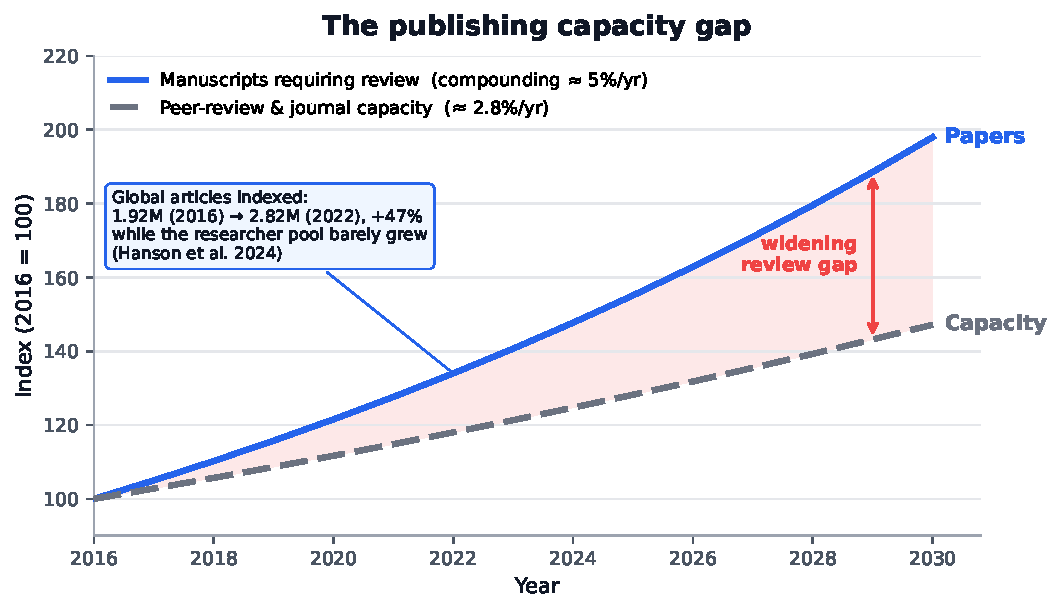
\includegraphics[width=0.86\textwidth]{capacity_gap.pdf}
  \caption{\small The structural mismatch AIDER addresses. Manuscript volume compounds at $\sim$5\%/yr while peer-review and journal capacity grow at $\sim$2.8\%/yr; the gap widens every year. Growth rates anchored to refs.~[14,15,17]; illustrative index, 2016\,$=$\,100.}
  \label{fig:gap}
\end{figure}

\textbf{(c) And the trust it produces is eroding.}
Paper mills now generate output in the hundreds of thousands; LLMs let low-quality and fabricated work be produced faster than human referees can screen it. \src{20} The traditional response --- review harder, by hand --- cannot scale to meet machine-speed production. A journal built \emph{for} the AI era, with transparency and automation at its core, can.

\begin{takeaway}
\textbf{In one line.} The old system is closed, expensive, and shut to individuals; the new flood of AI-assisted work is undocumented and far larger than human review can absorb. AIDER is built to be open, free, reproducible, fully documented, and \emph{scalable} --- precisely where the incumbents fail.
\end{takeaway}

% ═════════════════════════════════════════════════════════════════
\section{How AIDER Solves It}

Each AIDER requirement maps directly onto a problem above.

\begin{solvebox}
\begin{itemize}
\item \textbf{Mandatory open code + data + \texttt{reproduce.sh}} $\rightarrow$ kills the reproducibility \& reuse failure (1.1a). A paper is a living, runnable repository, not a dead PDF.
\item \textbf{Diamond open access --- \$0 to authors, \$0 to readers} $\rightarrow$ removes the pay-wall and APC barrier (1.1b, 1.1c). Sustained on free-tier infrastructure, not extraction.
\item \textbf{GitHub-native, individual-friendly submission} $\rightarrow$ gives independent researchers and developers a credible home (1.1c).
\item \textbf{Mandatory research-process log (AI transcripts, prompts, human decisions)} $\rightarrow$ converts the AI black box into an auditable record (1.2a).
\item \textbf{AI-augmented review pipeline (5 reviewer agents + human editor)} $\rightarrow$ scales review \emph{with} the paper flood instead of against it (1.2b), and absorbs the overflow.
\item \textbf{Living repository + continuous automated correction} $\rightarrow$ rebuilds trust through transparency, not gatekeeping (1.2c).
\end{itemize}
\end{solvebox}

% ═════════════════════════════════════════════════════════════════
\section{Who Else Is Trying --- and Why They Stall}

We are not the first to attempt open, free, reproducible publishing. The instructive part is \emph{why comparable efforts struggle to climb in prestige} --- and what that teaches us.

\renewcommand{\arraystretch}{1.32}
\begin{center}\small
\begin{tabular}{@{}p{2.9cm} p{6.3cm} p{6.0cm}@{}}
\toprule
\textbf{Venue} & \textbf{What it is} & \textbf{Where it stalls / lesson} \\
\midrule
\textbf{JOSS} \newline (J. Open Source Software) &
Diamond OA; peer review runs \emph{in the open as GitHub issues}; $>$3{,}500 papers; runs on \stat{$\sim$\$3/paper}. The closest model to us, and proof it works at scale. \src{21} &
Stuck on scope (software metapapers only) and \emph{shut out of Scopus/Web of Science despite repeated applications}. Free is solved; prestige is not. \\
\textbf{ReScience C} &
GitHub-native, diamond OA, replication-only journal. \src{22} &
Replication-only \stat{starves the pipeline} ($\sim$20 articles/yr, bursty). Lesson: publish primary research \emph{with} reproducibility, not reproducibility alone. \\
\textbf{Distill.pub} &
Celebrated interactive-ML journal. &
\stat{Discontinued in 2021} from \emph{volunteer burnout} ($>$50 hrs/article). Lesson: a heavy per-paper mandate must be \stat{automated}, not absorbed by people. \src{23} \\
\textbf{eLife} &
Prestigious OA journal; in 2023 moved to ``publish, then review'' with no accept/reject. &
In Oct 2024, Web of Science \stat{paused its impact factor} for ``decoupling publication from validation.'' Lesson: \stat{keep a clear accept/reject editorial gate}. \src{24} \\
\textbf{PLOS ONE} &
The original mega-journal (soundness-only review). &
Impact factor fell \stat{$\sim$40\%} from peak; output \stat{collapsed from 31{,}509 (2013)} as prestige slid. Lesson: \stat{volume without selectivity} decays. \src{25} \\
\textbf{MDPI / Hindawi} &
Fast, high-volume OA via special issues. &
\stat{Dozens of journals delisted}; Hindawi retracted \stat{$>$8{,}000 papers} (2023) from paper mills. Lesson: scaling \emph{must not} outrun quality control. \src{26} \\
\midrule
\textbf{Discrete Analysis} &
Diamond arXiv-overlay journal (Gowers), \stat{$\sim$\$10/submission}. &
\textbf{The proof it can be done:} \stat{indexed in Scopus, Web of Science \& DOAJ} --- credibility bought with a \stat{prestigious editorial board}, not money. \src{27} \\
\bottomrule
\end{tabular}
\end{center}

\begin{takeaway}
\textbf{The pattern.} Going free is easy; \emph{getting recognised} is the hard part, and it is gatekept by Scopus / Web of Science / DOAJ criteria that reward a \textbf{clear accept/reject review gate}, a \textbf{reliable publishing cadence}, persistent DOIs, ethics infrastructure, and a \textbf{credible editorial board}. The two failure modes are eLife (broke the validation gate $\to$ lost its impact factor) and PLOS/MDPI/Hindawi (scaled volume past quality $\to$ delisted). \textbf{Discrete Analysis proves a free journal \emph{can} reach top-tier indexing --- on the strength of its board, not its budget.} That is precisely the lane AIDER must drive.
\end{takeaway}

% ═════════════════════════════════════════════════════════════════
\section{The Plan --- Short Term (within 1 year)}

\subsection{Who are our users? (who submits)}

We do not need everyone --- we need the people the incumbents fail. Priority author segments:
\begin{itemize}
\item \textbf{AI-native researchers in energy} whose work \emph{is} code (ML for CFD, grid optimisation, RL control, PINNs, forecasting). Their reproducible artefacts are a liability elsewhere and an asset here.
\item \textbf{Independent developers \& unfunded / early-career researchers} priced out by APCs and shut out of prestige venues --- a solo contributor with great reproducible work.
\item \textbf{Authors of heavily AI-assisted research} who cannot get the AI process documented or credited in a traditional journal.
\item \textbf{The ``overflow''} --- sound papers bouncing off overloaded conventional journals because reviewers cannot be found, not because the work is weak.
\item \textbf{Our editorial board's own networks} --- a warm-start pipeline across Oxford, Imperial, Tsinghua, Kyoto, TU Delft, Harvard, and China Three Gorges.
\end{itemize}

\subsection{How do we attract reviewers?}

Reviewer scarcity is \emph{the} bottleneck that breaks everyone else (\S1.2b). We attack it from three sides:
\begin{itemize}
\item \textbf{AI agents carry the first pass.} Five reviewer agents (Claude, GPT, Gemini, Grok, Qwen) handle reproducibility checks, claim auditing, and reference verification --- so a human referee inherits a structured report, not a blank form. This is the only response that \emph{scales} with submission volume.
\item \textbf{We pay reviewers in credit, not cash.} Every review is published, signed, and citable --- fixing the ``reviewing is invisible and unrewarded'' problem that drives global reviewer fatigue. \src{19}
\item \textbf{Low time-cost \& a growing flywheel.} Because CI runs \texttt{reproduce.sh} and agents pre-screen, the marginal human review is fast; published authors are recruited as the next cohort of reviewers.
\end{itemize}

\subsection{12-month targets}
\begin{itemize}
\item Ship \textbf{Vol.~1 with $\ge$5 articles} (the ISSN \& DOAJ threshold), then push toward \textbf{10+}.
\item Secure the \textbf{ISSN}, register \textbf{Crossref DOIs}, and \textbf{apply to DOAJ} --- the table-stakes credibility floor every comparable venue clears early. \src{10,27}
\item Establish a \textbf{reliable publishing cadence} and a documented, public accept/reject review process --- the exact criteria Scopus/WoS reward (\S3).
\end{itemize}

% ═════════════════════════════════════════════════════════════════
\section{The Plan --- Long Term (3--5 years)}

\subsection{The destination: a Nature/Science-tier venue for the AI era}

The aspiration is genuine prestige --- but we get there on a different road than the incumbents, because our differentiator is structurally stronger in this era: \textbf{the highest-trust, fully reproducible, fully AI-documented venue, at a moment when trust in the literature is collapsing}. The indexing ladder is well defined:
\begin{center}\small
\renewcommand{\arraystretch}{1.2}
\begin{tabular}{@{}ll@{}}
\textbf{Year 1} & ISSN $\to$ Crossref DOIs $\to$ DOAJ listing (the credibility floor) \\
\textbf{Year 1--2} & Google Scholar / OpenAlex coverage; steady cadence; Web of Science ESCI \\
\textbf{Year 2--3} & Scopus (requires a publication track record + regular schedule) \\
\textbf{Year 3--5} & Web of Science SCIE + first Journal Impact Factor; aim for field-leading status \\
\end{tabular}
\end{center}
We will \textbf{not} repeat eLife's mistake (we keep a clear editorial accept/reject gate) nor MDPI's (selectivity scales with volume). We \emph{will} copy Discrete Analysis: let a credible board and reproducibility-first rigour, not money, buy the prestige. \src{24,26,27}

\subsection{The moat: automation \& reproducibility}

The AI-augmented pipeline is not a convenience --- it is the moat. It lets us absorb the over-production that is \emph{breaking} traditional journals, while a 100\%-reproducible, fully-logged corpus becomes the most trustworthy body of work in the field. Automation is also what saves us from Distill's fate (burnout) and ReScience's (starved pipeline). \src{23}

\subsection{Money: stay diamond, forever}

\begin{takeaway}
\textbf{Principle: readers never pay, authors never pay.} The \$19\,bn incumbent industry runs on 30--40\% margins extracted from free labour. \src{6,8} We refuse that model.
\end{takeaway}
\begin{itemize}
\item \textbf{Costs are near-zero by design.} GitHub Pages (hosting), GitHub Actions (CI), Zenodo (archival + DOIs), volunteer editors, and AI review at near-zero marginal cost. Comparable diamond journals run on \stat{$<$\$10{,}000/year}; JOSS runs on \stat{$\sim$\$3/paper}. \src{10,21}
\item \textbf{The one small, optional spend} is Crossref membership ($\sim$\$275/yr) if we want to mint our own DOIs --- Zenodo DOIs are free and sufficient until then.
\item \textbf{If we ever need funds}, the diamond-OA-aligned routes (institutional grants, library-consortia support such as the EU's DIAMAS/CRAFT-OA programmes, foundation grants like JOSS's Sloan funding) fund \emph{infrastructure} --- never a paywall, never an APC. \src{10}
\item \textbf{No legal entity, no revenue, no APCs} keeps the project compatible with everyone's day job and visa status, and keeps incentives clean.
\end{itemize}

% ═════════════════════════════════════════════════════════════════
\section{Roadmap \& Current Status}

\renewcommand{\arraystretch}{1.25}
\begin{center}\small
\begin{tabular}{@{}p{2.4cm} p{8.6cm} p{2.6cm}@{}}
\toprule
\textbf{When} & \textbf{Milestone} & \textbf{Status} \\
\midrule
Feb 2026 & Journal founded; website, submission pipeline, editorial policies built & \textcolor{green}{\textbf{Done}} \\
Feb 2026 & End-to-end submission \& AI-review pipeline tested & \textcolor{green}{\textbf{Done}} \\
Mar 2026 & First paper published (Foundation Models for Clean Energy), Zenodo DOI & \textcolor{green}{\textbf{Done}} \\
Mar 2026 & ISSN application submitted to the British Library (ISSN UK Centre) & \textcolor{amber}{\textbf{Held on file}} \\
Jun 2026 & \textbf{Four papers published, fifth under review} & \textcolor{green}{\textbf{Done}} \\
Jun 2026 & \textbf{First editors' online meetup (today)} & \textcolor{accent}{\textbf{Now}} \\
Q2--Q3 2026 & Ship Vol.~1 with $\ge$5 articles; recontact ISSN; Crossref; apply to DOAJ & \textcolor{ink3}{Planned} \\
Late 2026 & Google Scholar / OpenAlex coverage; grow to 10+ papers & \textcolor{ink3}{Planned} \\
2027+ & Scopus, then Web of Science / Impact Factor & \textcolor{ink3}{Planned} \\
\bottomrule
\end{tabular}
\end{center}

\textbf{Where we stand today.} \stat{4 papers published} (Vol.~1, No.~1--4), a \stat{5th under review}; \stat{ISSN held on file} at the British Library, to be assigned once Vol.~1 ships 5+ articles; \stat{9 founding editors} and \stat{5 AI reviewer agents} active.

\subsection*{Published so far}
\begin{enumerate}
\item \emph{Foundation Models for Clean Energy Systems: A Scoping Review and Deployment Framework} --- J. Jiang (Oxford). Vol.~1(1). DOI: 10.5281/zenodo.18902064.
\item \emph{Advancing Clean Energy Conversion through Electrocatalysis: High-Efficiency Oxygen Reduction in Sustainable Fuel Cells} --- J. Wu (Kyoto). Vol.~1(2).
\item \emph{A Data-Driven Design Strategy for Next-Generation Lithium Batteries} --- J. Wu (Kyoto). Vol.~1(3).
\item \emph{A Pareto Frontier between Equilibrium Fidelity and Reversed-Flow Sign Accuracy in Neural Wall Function Formulations} --- J. Jiang (Oxford). Vol.~1(4).
\end{enumerate}

\subsection*{Founding editorial board}
\begin{center}\small
\renewcommand{\arraystretch}{1.15}
\begin{tabular}{@{}ll@{}}
Jianou Jiang (Founding Editor) & University of Oxford \\
Raul Adriaensen & Imperial College London \\
Dr.\ Feng Wei & CAICT, Ministry of Industry \& Information Technology \\
Dr.\ Yadong Han & Tsinghua University \\
Qian Wang & China Three Gorges Renewables \\
Shixin Huo & Delft University of Technology \\
Jingda Wu & Kyoto University \\
Xinle Dai & Harvard University \\
Xiaolan Ke & Harvard University \\
\end{tabular}
\end{center}
\emph{AI reviewer agents:} Claude (Anthropic), GPT (OpenAI), Gemini (Google DeepMind), Grok (xAI), Qwen (Alibaba Cloud).

% ═════════════════════════════════════════════════════════════════
\section*{References}
{\footnotesize\color{ink2}\raggedright
\begin{enumerate}[leftmargin=1.6em, itemsep=1.5pt]
\item Baker, M. (2016). 1{,}500 scientists lift the lid on reproducibility. \emph{Nature} 533, 452--454.
\item Stodden, V., Seiler, J., \& Ma, Z. (2018). An empirical analysis of journal policy effectiveness for computational reproducibility. \emph{PNAS} 115(11), 2584--2589.
\item Vines, T. H., et al. (2014). The availability of research data declines rapidly with article age. \emph{Current Biology} 24(1), 94--97.
\item \emph{(reserved)}
\item Else, H. (2020). Nature journals reveal terms of landmark open-access option (\euro9{,}500 / US\$11{,}390 APC). \emph{Nature} news, 24 Nov 2020.
\item Johnson, R., Watkinson, A., \& Mabe, M. (2018). \emph{The STM Report}, 5th ed. STM Association ($\sim$\$19.8\,bn market).
\item Larivière, V., Haustein, S., \& Mongeon, P. (2015). The Oligopoly of Academic Publishers in the Digital Era. \emph{PLOS ONE} 10(6), e0127502.
\item RELX / Elsevier (2024). \emph{2023 Annual Results} (38\% STM operating margin).
\item Butler, L.-A., et al. (2024). Estimating global article processing charges paid to six publishers, 2019--2023. arXiv:2407.16551.
\item Bosman, J., et al. (2021). \emph{OA Diamond Journals Study}. Science Europe / cOAlition S (17{,}000--29{,}000 diamond journals; 8--9\% of articles; median $\sim$23/yr).
\item Kobak, D., et al. (2024). Delving into LLM-assisted writing in biomedical publications through excess vocabulary. arXiv:2406.07016 (\emph{Science Advances}).
\item Liang, W., et al. (2024). Monitoring AI-Modified Content at Scale: ChatGPT's impact on AI conference peer reviews. ICML 2024 / arXiv:2403.07183.
\item Walters, W. H., \& Wilder, E. I. (2023). Fabrication and errors in the bibliographic citations generated by ChatGPT. \emph{Scientific Reports} 13, 14045.
\item Hanson, M. A., et al. (2024). The strain on scientific publishing. \emph{Quantitative Science Studies} 5(4), 823--843 / arXiv:2309.15884.
\item Bornmann, L., Haunschild, R., \& Mutz, R. (2021). Growth rates of modern science. \emph{Humanities \& Social Sciences Communications} 8, 224.
\item arXiv submission statistics (2024). \href{https://info.arxiv.org/help/stats/}{info.arxiv.org/help/stats} \& arXiv blog, Nov 2024 (record 24{,}226 submissions, Oct 2024).
\item Mabe, M. (2003). The growth and number of journals. \emph{Serials} 16(2) ($\sim$3.5\%/yr); cf.\ Scopus journal counts.
\item Kovanis, M., et al. (2016). The Global Burden of Journal Peer Review in the Biomedical Literature. \emph{PLOS ONE} 11(11), e0166387.
\item Publons / Clarivate (2018). \emph{Global State of Peer Review 2018}.
\item Van Noorden, R. (2023). More than 10{,}000 research papers were retracted in 2023 --- a new record. \emph{Nature} 624, 479--481.
\item Smith, A., et al. \emph{Journal of Open Source Software} --- \href{https://joss.theoj.org/about}{joss.theoj.org} (open GitHub-issue review; $>$3{,}500 papers; $\sim$\$3/paper; not in Scopus/WoS).
\item \emph{ReScience C} --- \href{http://rescience.github.io/}{rescience.github.io} (GitHub-native replication journal; low organic volume).
\item Distill (2021). \emph{Distill Hiatus}. \href{https://distill.pub/2021/distill-hiatus/}{distill.pub/2021/distill-hiatus} (volunteer burnout; $>$50 hrs/article).
\item eLife (2024). Update on eLife's indexing status at Web of Science (SCIE paused, 23 Oct 2024); Van Noorden / Retraction Watch (13 Nov 2024).
\item PLOS ONE impact-factor \& output trajectory: Scholarly Kitchen (2013--2017); \emph{Inside Higher Ed} (2017); Wikipedia ``PLOS One'' (peak 31{,}509 articles, 2013).
\item MDPI Web of Science delistings (IJERPH \& JRFM, Feb 2023), MDPI announcements; Van Noorden, R. (2023), \emph{Nature} 624 (Hindawi $>$8{,}000 retractions).
\item Gowers, T. (2015); \emph{Discrete Analysis} --- arXiv-overlay diamond journal; indexed in Scopus, Web of Science \& DOAJ.
\end{enumerate}
}

\clearpage
\vspace*{\fill}
\begin{center}
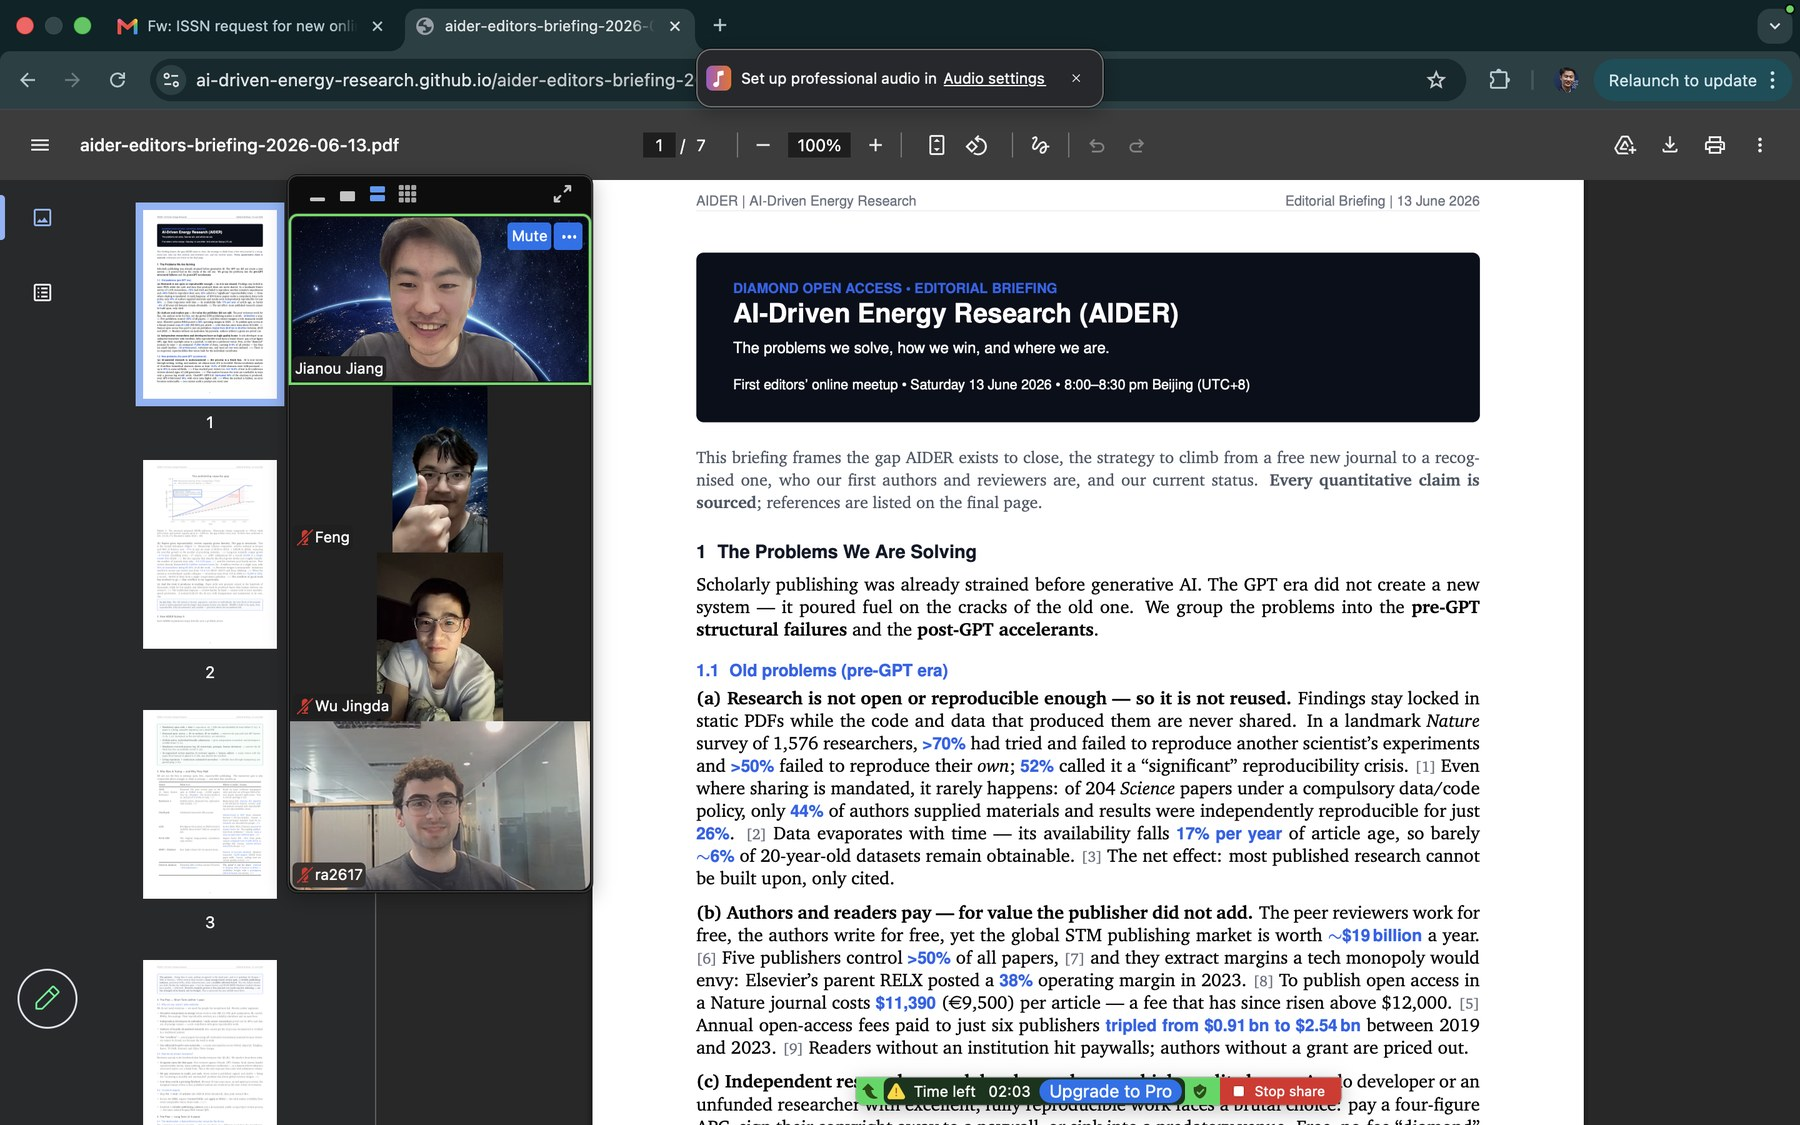
\includegraphics[width=0.78\textwidth]{group_photo.jpg}\\[8pt]
{\footnotesize\color{ink3} The AIDER editorial team at the first online meetup --- 13 June 2026.}\\[16pt]
{\footnotesize\color{ink3} Published by AI-Driven Energy Research (AIDER), Oxford, United Kingdom. All content CC-BY 4.0.\\ \href{https://ai-driven-energy-research.github.io/}{ai-driven-energy-research.github.io}}
\end{center}
\vspace*{\fill}

\end{document}
